\documentclass{../template/tp}
\usepackage[utf8x]{inputenc}

\usepackage[frenchb]{babel}
\usepackage[T1]{fontenc}

\usepackage{graphicx}
\usepackage{amssymb}
\usepackage{amsmath}
\usepackage{wasysym} %smiley
\usepackage{hyperref}% hyperliens
\usepackage{tikz}
\usetikzlibrary{babel,positioning,calc}
\usepackage[]{circuitikz}
\usepackage{textcomp}
% \usepackage{minted}
\usepackage[long]{datetime}
\usepackage{gensymb} % \ohm, celsius
\usepackage{framed}
\usepackage{pdfpages}
\usepackage{todo}
\usepackage{fancyhdr}
\usepackage{caption} % subfigure
\usepackage{subcaption} % subfigure
\usepackage{pgfplots} % axis
\usepackage{siunitx} 

\graphicspath{{./Figures/}}

% \langexam{frenchb}

\newboolean{koriG}
\ifx\koriG\undefined
\correction{false}
\else
\correction{true}
\fi

% \correction{false}
%  \correction{true}

%% fancy header & foot
\pagestyle{fancy}
\lhead{[ELEC-H-301] Électronique appliquée\\ TP \no 6 : Problèmes contextualisés\ifthenelse{\boolean{corrige}}{~-- Corrigé}{}}
\rhead{v2.0.2\\ page \thepage}
\cfoot{}
%%

\pdfinfo{
/Author (ULB -- BEAMS)
/Title (TP 6 ELEC-H-301, Problèmes contextualisés)
/ModDate (D:\pdfdate)

}
\hypersetup{
pdftitle={TP 6 [ELEC-H-301] Électronique appliquée : Problèmes contextualisés},
pdfauthor={ULB - BEAMS  },
pdfsubject={Problèmes contextualisés}
}

\author{The Fantastic Four}

\begin{document}

\tptitle{ELEC-H-301~: Électronique appliquée}{Séance 6~: Problèmes contextualisés}

% \todo{Arranger l'ordre des exercices}

Cette séance d'exercices a pour objectifs de vous apprendre à:
\begin{itemize}
\item Bien contextualiser les problèmes d'électronique vus cette année.
\item Sélectionner les bonnes méthodes de résolution de circuits électroniques.
\end{itemize}


























\section*{Transistor -- Janvier 2019}

On désire dimensionner un étage amplificateur à l'aide du circuit suivant.
Le gain à vide de cet étage est de $ 50~dB $.
On dispose d'une alimentation continue $ V_{DC} $ de $ 10~V $ et d'un transistor BSH105.
La résistance $ R_{d} $ vaut $ 90~\Omega $.
\begin{center}
    \begin{circuitikz}[scale=1]\draw
        (0,1) to [short,o-] (9,1)
              to [battery, l=$ V_{DC} $, invert](9,6)
        (4,6) to [short] (9,6)
        (0,3) to [short,o-] (1,3)
        (0,3) to [open, v_<=$ V_{in} $]  (0,1)
        (1,3) to [C=$ C_{1} $ ](1.5,3)
        (1.5,3) to [short,-*] (2,3)
        (2,6) to [short] (4,6)
        (2,6) to [R, l_=$ R_{1} $] (2,3)
              to [R, l_=$ R_{2} $] (2,1)
        (4,3) node[nfet] (mos) {}
        (mos.G) to [short] (2,3)
        (mos.D) to (4,4) to [R, l_=$ R_{d} $] (4, 6)        
        (mos.D) to [short,-*](4,3.5)  to [short] (4.25,3.5)
        (mos.S) to [short] (4,1)
        (mos.S) -- (mos.B) %source to bulk connection
        (4.25,3.5) to [C, l^=$ C_{2} $] (6,3.5) 
                   to [short](6,3.5)
         %          to [short,-o](6.5,3.5)node [anchor=south] {Out} 
        (6,3.5) to [resistor, l_=$ R_{ch} $, *-*] (6,1)
        (6.5,3.5) to [open,v^<=$ V_{out} $] (6.5,1)
        (0,0.5) -- (0,1) node[ground]{}
    ;\end{circuitikz}
\end{center}
\begin{figure}[h!]
    \centering
    
    \begin{subfigure}[b]{0.49\linewidth}
        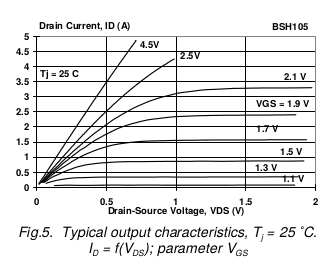
\includegraphics[width=\linewidth]
            {datasheet_transistor_sortie.png}
        \caption{}
        \label{fig:Sortie}
    \end{subfigure}%
    ~
    \begin{subfigure}[b]{0.49\linewidth}
        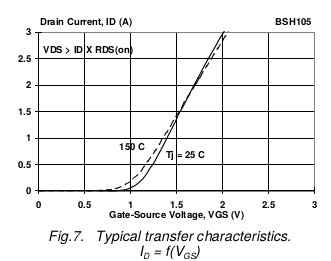
\includegraphics[width=\linewidth]
            {datasheet_transistor_transfer.png}
        \caption{}
        \label{fig:Transfer}
    \end{subfigure}

    \begin{subfigure}[b]{0.49\linewidth}
        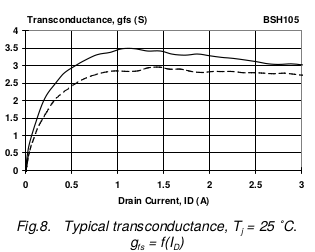
\includegraphics[width=\linewidth]
            {datasheet_transistor_transconductance.png}
        \caption{}
        \label{fig:Transconductance}
    \end{subfigure}
    
    \caption{Extrait datasheet BSH105.}

\end{figure}

\Question
{
    Dessinez le schéma équivalent à petits signaux pour des fréquences telles que les effets dûs aux condensateurs \textbf{ne} sont \textbf{pas} négligeables.
}{
    \begin{center}
      \begin{circuitikz}[scale=0.8]\draw
          % Left side
          (0,0) to [open, v^>=$ V_{in} $, ]  (0,3)
                  to [C, l=$ C_{1} $, o-] (2,3)
                to [short, -o] (4,3)
                to [open, v^<=$ V_{g} $](4,0)
            (2,3) to [R, l_=$ R_{1} $] (2,0)
            (3,3) to [R, l=$ R_{2} $] (3,0)
            
            % Right side
            (0,0) to [short, o-o] (12,0)
                  to [open, v>=$ V_{out} $](12,3)
                  to [short, o-] (11,3)
                  to [C, l_=$ C_{2} $] (9,3)
                  to [short, -](6,3)
                  to [cI=$ g_m \cdot V_{g} $] (6,0)
            (9,3) to [R, l_=$ R_{D} $] (9,0)
            (11,3) to [R, l=$ R_{ch} $] (11,0)
        ;\end{circuitikz}
    \end{center}
}

\Question
{
    Donnez l'expression du gain \textbf{à vide} de ce montage à très haute fréquence tel que les effets dûs aux condensateurs soient négligeables.
    Déduisez-en la valeur de la transconductance pour le gain donné.
}{
    Le gain est donné par:
    \[G = - g_{m} R_{d}\]
    
    Un gain de $ 50~dB $ correspond à un gain de $ 10^{50/20} = 316 $ en naturel.
    
    \[ g_{m} = \frac{|G|}{R_{d}} = 3.5~S \]
}

\Question
{
    Trouvez le $ V_{gs} $ correspondant. Justifiez graphiquement.
}{
    On trouve le courant de sortie $ I_{D} \approx 1~A $ grâce à la Figure~\ref{fig:Transconductance} pour $ g_m = 3.5~S $.
    Le $ V_{gs} $ est donné par la Figure~\ref{fig:Transfer} et vaut approximativement $ 1.4~V $
    
}

\Question
{
    Déterminez l'expression de la résistance d'entrée, en négligeant l'effet du condensateur.
}{
    \[ R_{in} = R_{1} // R_{2} = \frac{R_{1} R_{2}}{R_{1} + R_{2}} \]
}

\Question
{
    Dimensionnez $ R_{1} $ et $ R_{2} $ pour avoir une résistance d'entrée de $ 5~k\Omega $. Si vous n'avez pas trouvé $ V_{gs} $ considérez $ V_{gs} = 1.7~V $.
}{
    On a:
    \[
        R_{in} = \frac{R_{1} R_{2}}{R_{1} + R_{2}} = 5~k\Omega
        \qquad\text{et}\qquad
        V_{gs} = \frac{R_{2}}{R_{1} + R_{2}} V_{DC} = 1.4~V
    \]
    Par conséquent:
    \[
        \left\{ 
            \begin{array}{ll}
                R_{1} &= R_{in} \frac{V_{DC} }{ V_{gs} } = 35,7~k\Omega\\
                R_{2} &= \frac{ R_{in} R_{1} }{ R_{1} - R_{in} } = 5,8~k\Omega
            \end{array}
        \right.
    \]
    
}

\clearpage





















\section*{Analyse fréquentielle -- Janvier 2019}

\Question
{
Réalisez le tracé asymptotique des courbes de Bode de la fonction de transfert suivante.
Listez clairement les pôles et zéros identifiés, ainsi que leur degré respectif.
Légendez clairement les repères.

\[H(p) = \frac{10^3 \cdot (p + 10^2)^3 \cdot(p+10^4)}{p \cdot (p+10^3) \cdot (p+10^5)^3}\]

\begin{center}
\begin{tikzpicture}
\begin{axis}[
    width=10cm,
    % height=5cm,
    xmode=log, ymode=log,
    xmin=1e-1, xmax=1e8,
    ymin=1e-1, ymax=1e7,
    grid=both,
    major grid style={black!50},
    yticklabels={,,},
    xticklabels={,,}
]
\end{axis}
\end{tikzpicture}
\end{center}

\begin{center}
\begin{tikzpicture}
\begin{axis}[
    width=10cm,
    % height=5cm,
    xmode=log,
    xmin=1e-1, xmax=1e8,
    ymin=0, ymax=4,
    grid=both,
    major grid style={black!50},
    yticklabels={,,},
    xticklabels={,,}
]
\end{axis}
\end{tikzpicture}
\end{center}
% Question
}{
Passons d'abord à la forme canonique :
\begin{align*}
H(p) & = \frac{10^3 \cdot (p + 10^2)^3 \cdot(p+10^4)}{p \cdot (p+10^3) \cdot (p+10^5)^3} \\
     & = \frac{10^3 \cdot 10^6 \cdot (1+\frac{p}{10^2})^3 \cdot 10^4 \cdot (1+\frac{p}{10^4})}{p \cdot 10^3 \cdot (1 + \frac{p}{10^3}) \cdot 10^{15} \cdot (1 + \frac{p}{10^5})^3} \\
     & = \frac{10^{-5} \cdot (1+\frac{p}{10^2})^3 \cdot (1+\frac{p}{10^4})}{p \cdot (1 + \frac{p}{10^3}) \cdot (1 + \frac{p}{10^5})^3} \\
\end{align*}


\begin{itemize}
\item Zéros : $10^2$ (degré 3) et $10^4$ (degré 1)
\item Pôles : $0$ (degré 1), $10^3$ (degré 1) et $10^5$ (degré 3)
\item $A_o = 10^{-5}$
\end{itemize}

\begin{center}
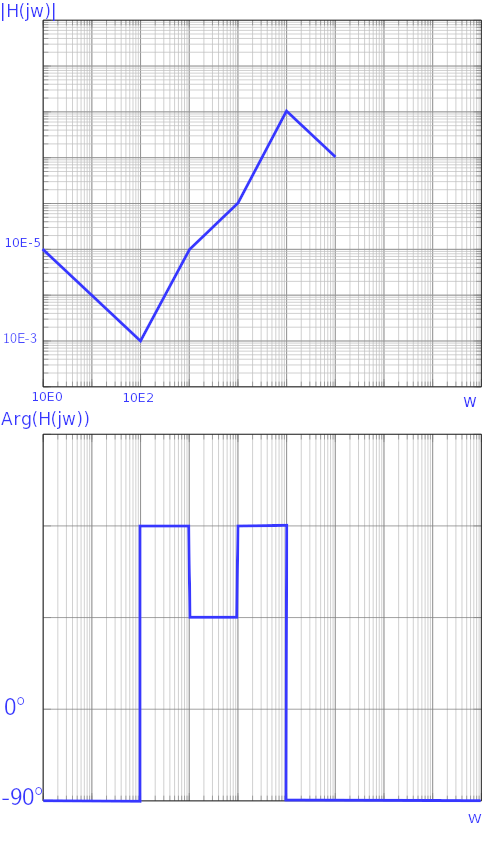
\includegraphics[width=10cm]{elech301_bode.png}
\end{center}
}
\clearpage















\section*{Accordeur électronique -- Janvier 2020}

Nous aimerions réaliser un accordeur électronique fonctionnant de la manière suivante~: une note est jouée devant le micro du système qui indique ensuite à l'aide de trois LED à l'utilisateur si elle est trop basse, trop aiguë ou juste.
Pour y parvenir, le signal est d'abord séparé selon deux pistes : l'une au travers d'un filtre passe-bas réglé à la fréquence de référence, l'autre passe-haut à la même fréquence.
Le bloc de lissage adjacent permet ensuite de conserver le valeur maximale de la sinusoïde entre deux période du signal.

Le schéma suivant vous donne quelques indications quant à sa conception~:

\begin{center}
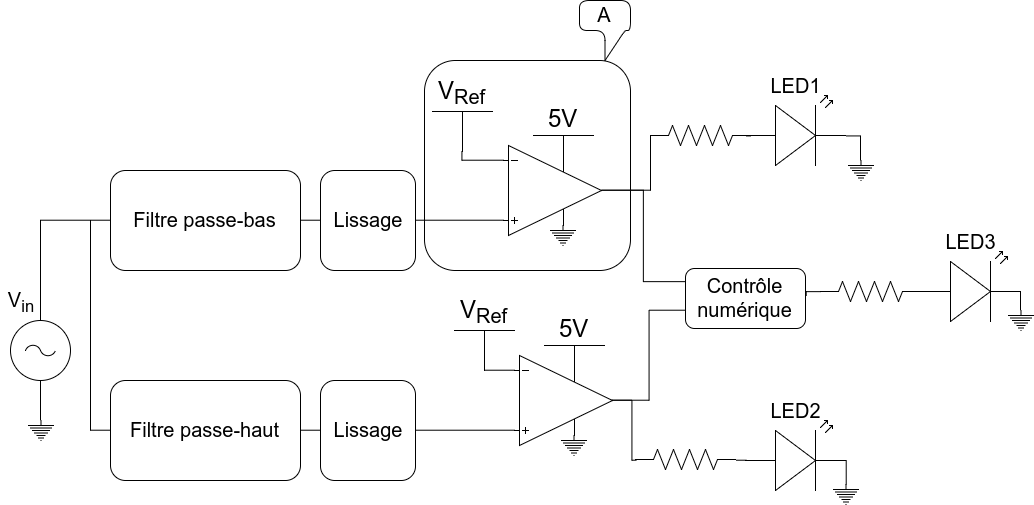
\includegraphics[width=\textwidth]{elech301_schema-bloc_mystere.png}
\end{center}

Votre tâche consiste à comprendre, concevoir et dimensionner ce système et les blocs le composant.

\Question
{
Notre accordeur utilise comme note de référence le $la_3$ à 440 Hz. Dessinez et dimensionnez les deux filtres passe-haut et passe-bas d'ordre 1 à l'entrée du montage.
}
{
\begin{enumerate}
\item Filtre passe-haut, RC ou RL.

    \begin{itemize}
    \item RC avec $\omega_C = \frac{1}{RC} = 2\pi \cdot 440$. Si l'on choisit $R = 1k\Omega$, $C = 361.7 nF$.
    
    \begin{circuitikz} \draw
    (0,0)   node[ground]{}
            to[american voltage source, v=$V_{in}$, invert] (0,3)
            to[C, l=$C$] (3,3)
            (3,0) to[R, l=$R$, v=$V_{out}$] (3,3)
            (3,0)--(0,0)
    ;
    \end{circuitikz}
    
    \item RL avec $\omega_C = \frac{R}{L} = 2\pi \cdot 440$. Si l'on choisit $R = 1k\Omega$, $L = 361.7 mH$.
    
    \begin{circuitikz} \draw
    (0,0)   node[ground]{}
            to[american voltage source, v=$V_{in}$, invert] (0,3)
            to[R, l=$R$] (3,3)
            (3,0) to[L, l=$L$, v=$V_{out}$] (3,3)
            (3,0)--(0,0)
    ;
    \end{circuitikz}
    \end{itemize}


\item Filtre passe-bas, RC ou RL.

    \begin{itemize}
    \item RC avec $\omega_C = \frac{1}{RC} = 2\pi \cdot 440$. Si l'on choisit $R = 1k\Omega$, $C = 361.7 nF$.
    
    \begin{circuitikz} \draw
    (0,0)   node[ground]{}
            to[american voltage source, v=$V_{in}$, invert] (0,3)
            to[R, l=$R$] (3,3)
            (3,0) to[C, l=$C$, v=$V_{out}$] (3,3)
            (3,0)--(0,0)
    ;
    \end{circuitikz}
    
    \item RL avec $\omega_C = \frac{R}{L} = 2\pi \cdot 440$. Si l'on choisit $R = 1k\Omega$, $L = 361.7 mH$.
   
    \begin{circuitikz} \draw
    (0,0)   node[ground]{}
            to[american voltage source, v=$V_{in}$, invert] (0,3)
            to[L, l=$L$] (3,3)
            (3,0) to[R, l=$R$, v=$V_{out}$] (3,3)
            (3,0)--(0,0)
    ;
    \end{circuitikz}
    \end{itemize}
\end{enumerate}
}


\Question
{
Dessinez un montage effectuant l'opération de lissage décrite dans l'introduction.
}
{
Un montage avec une seule diode est suffisant, mais un pont de Wien est aussi possible.

\begin{circuitikz}\draw
    (0,0) to [sV, l=$V_{ac}$] (0,3)
    to [Do] (5,3)
    to [european resistor,l=$R_{Ch}$] (5,0) to (0,0)
    (4,3) to [eC,l_=$C$, *-*] (4,0)
    (6,3) to [open, v^<=$V_{charge}$] (6,0)
;\end{circuitikz}

Étant donné qu'on souhaite lisser la tension à l'entrée de l'ampli-op, la charge est nécessaire pour que les charges accumulées dans le condensateur puissent y circuler.
En l'absence de cette charge, le condensateur ne peut pas se décharger et ne sert donc pas son rôle de lissage.
De plus, le condensateur doit être polarisé pour que les charges puissent s'y accumuler lors des alternances positives et se décharger lors des alternances négatives.
}


\Question
{
Comment appelle-t-on le bloc A~? Quel est son rôle et quelle serait une valeur pertinente pour $V_{Ref}$, si $V_{in}$ a une amplitude maximale de 1~V ?
Justifiez votre réponse.
}
{
Il s'agit d'un montage comparateur.
Pour rappel, il fonctionne en mode différentiel, sans rétroaction. Lorsque $V_+ > V_-$, $V_{out} = 5 V$ et lorsque $V_+ < V_-$, $V_{out} = 0 V$.

La \texttt{LED1} doit être allumée si la fréquence de $V_{in}$ est trop basse, donc si cette fréquence est plus basse que la fréquence de coupure du filtre passe-bas.
On peut donc fixer $V_{Ref} = \frac{1}{\sqrt{2}} = 0.7 V$.
}


\Question
{
Le bloc de contrôle numérique permet de déterminer quand la \texttt{LED3} est allumée ou non.
Il est composé de deux entrées et d'une sortie, et doit fonctionner de la façon suivante~:
La LED ne doit s'allumer que si les deux autres sont éteintes et si l'une des deux autres est allumée, la \texttt{LED3} doit être éteinte. Une fois que la \texttt{LED3} a été allumée, elle doit le rester même si la note n'est plus jouée à l'entrée du diapason.

Dessinez le montage répondant à ce cahier des charges en utilisant des portes logiques et des organes mémoires si nécessaire.
}
{
\begin{center}
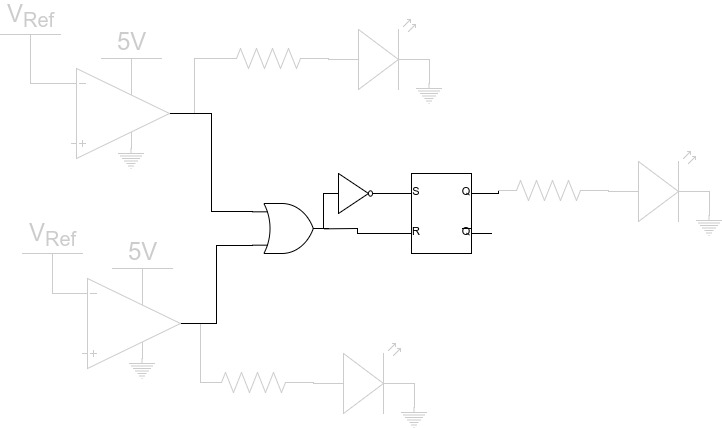
\includegraphics[width=\textwidth]{elech301_schema-bloc_logic.jpg}
\end{center}

Notez que le bistable n'est pas nécessaire au bon fonctionnement du montage~; la combinaison d'une porte \texttt{OR} avec une porte {NOT} est suffisante.
}


Les trois LED ont les mêmes caractéristiques dont vous pouvez trouver un extrait au travers des courbes suivantes~:

\begin{center}
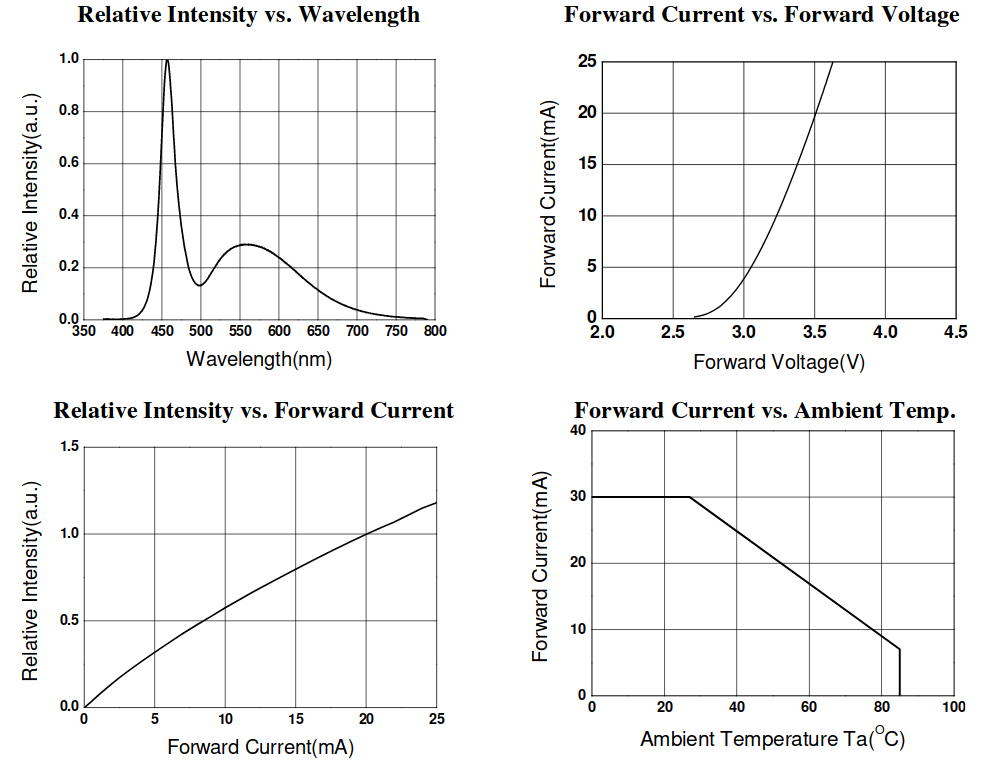
\includegraphics[width=.8\textwidth]{led_datasheet.png}
Bien qu'une simple porte \texttt{NOR} fasse l'affaire.
\end{center}

\Question
{
\begin{enumerate}
\item Dimensionnez la résistance connectée à l'anode de la LED afin qu'elle s'illumine avec une intensité lumineuse relative (\textit{Relative Intensity}) de 1 lorsqu'on applique une tension de 5 V à l'autre borne de la résistance.

\item Vous n'avez malheureusement sous la main qu'une résistance de $1 k\Omega$.
Sachant que la puissance maximale que la diode peut dissiper est de 100~mW, la LED ...
    \begin{itemize}
    \item[$\square$]... s'allume normalement. Déterminez sa nouvelle intensité lumineuse.
    \item[$\square$]... s'allume brièvement avant de brûler. Déterminez la puissance qu'elle dissipe brièvement avant d'être inutilisable.
    \item[$\square$]... se transforme spontanément en or. Déterminez comment reproduire ce phénomène à l'échelle industrielle.
    \end{itemize}
\textit{Note : Cochez la bonne réponse et ne répondez qu'à la sous-question correspondante.}
\end{enumerate}

}
{
\begin{enumerate}
\item L'une des difficultés de l'exercice est de comprendre le circuit équivalent à la sortie du montage.
Étant donné que l'étage à AOP sature sur $0 V$ ou $5 V$, on peut conceptuellement le remplacer par une source de tension continue $E$ de $0 V$ ou $5 V$.
On obtient alors une maille $E - V_R - V_D = 0$.
En suivant les différentes courbes, on constate qu'une intensité lumineuse relative de 1 correspond à un courant de 20 mA pour une tension de 3.5 V aux bornes de la diode.
Pour une sortie d'AOP comparateur de $5 V$, nous avons une maille d'équation $5V - V_R - V_D = 0$, avec $V_R = i \cdot R$.
Étant donné que $V_D = 3.5 V$ et que $i = 20 mA$, on trouve $R = 75 \Omega$.


\item La LED s'allume normalement. Une droite de charge permet de déterminer qu'elle est parcourue par un courant d'environ 3 mA sous une tension d'environ 3 V, entraînant une intensité lumineuse relative d'environ 0.2 et une puissance dissipée de $3 V \cdot 3 mA = 9 mW$.

Attention ! Cette question ne signifie pas que la diode dissipe 100 mW quand on utilise une résistance $1 k\Omega$.
De plus, on ne peut pas utiliser la relation $P = R\cdot I^2$ pour une diode, puisqu'il s'agit de l'expression de la puissance dissipée par une résistance.
\end{enumerate}
}

\clearpage





















\section*{Dimensionnement d'une amplification -- Janvier 2020}

On souhaite créer un circuit d'amplification pour un signal sinusoïdal dont la plage de fréquence s'étend de \si{20}{kHz} à \si{40}{kHz}.
Ce signal peut être représenté par une sinusoïde d'amplitude \si{1}{mV} centré sur zéro produite par un générateur dont la résistance de sortie est \si{1}{k\ohm}.
En sortie, le signal amplifié doit avoir une amplitude de \si{12}{V} et sera connecté à une charge de \si{200}{\ohm}.
Le signal de sortie peut être déphasé par rapport au signal d'entré.
\begin{center}
\begin{circuitikz}[scale=0.8]
    \draw
        (0,0) node[ground]{}
            to[sinusoidal voltage source, v=$V_{in}$] (0,3)
            to[R, l=\si{1}{k\ohm}] (2,3)
            to[short] (3,3)
            to[open] (7,3)
            to[short] (10,3)
            to[R, l_=\si{200}{\ohm}, v^<=$ V_{out} $](10,0)
            to[short] (7,0)
            to[open] (3,0)
            to[short] (0,0)
        (0,4.3) node[anchor=south] {Générateur}
        (5,4.3) node[anchor=south] {Amplification}
        (10,4.3) node[anchor=south] {Sortie}
        (5,1.2) node[anchor=south] {{\large ?}}
    ;
    \draw[thick] (3, 3.5) -- (7, 3.5) -- (7, -0.5) -- (3, -0.5) -- (3, 3.5);
    \draw[dotted](-2,-1)--(-2,4)--(2,4)--(2,-1)--(-2,-1);
    \draw[dotted](8.3,-1)--(8.3,4)--(11.7,4)--(11.7,-1)--(8.3,-1);
\end{circuitikz}
\end{center}
\begin{table}[h]
    \centering
    \renewcommand{\arraystretch}{1.3}
    %\resizebox{\columnwidth}{!}{%
    \begin{tabular}{|l|c|c|c|r|}
        \hline
        Ampli-op & $ I_{out, max} [mA]$ & $ A.B_{W} [MHz]$ & Alimentation [V]& Prix [€]\\ \hline
        %     & [mA]& [MHz]  & [V] & [€] \\ \hline
        \texttt{MCP6V36T}  & 21   & 0.3 & 1,8 à 5,5             & 0,71\\ \hline
        \texttt{OPA548T}   & 5000 & 1   & $\pm 4$ à $\pm 30$    & 13,76\\ \hline
        \texttt{UA741CD}   & 25   & 1   & $\pm 9$ à $\pm 15$    & 0,3\\ \hline
        \texttt{AD8021ARZ} & 75   & 200 & $\pm 2,25$ à $\pm 12$ & 3,52\\ \hline
    \end{tabular}
    %}
\end{table}

\Question
{
    Dimensionnez le circuit d'amplification de la manière la plus économique possible. 
    Vous ne devez considérer que le prix des ampli-op listés ci-dessus.
    Le prix de tous autres composants (résistances,...) est négligeable. 
    %Vous ne devez pas considérer le prix des résistances et autres composants basiques.
    Proposez des valeurs de résistance réalistes et dessinez le schéma de ce circuit.\\
    \textit{Remarque: Commencez par établir la liste des contraintes du problème.}
}
{
    Les contraintes sont:
    \begin{itemize}
        \item Le gain total est $ G = \frac{\si{12}{V}}{\si{1}{mV}} = 12000 $,
        \item l'impédance d'entrée doit être supérieure à \si{1}{k\ohm},
        \item le dernier étage doit être capable de fournir un courant de sortie supérieur à 
            $ \frac{ \si{12}{V} }{ \si{200}{\ohm} } = \si{60}{mA} $.
    \end{itemize}
    ~\\

    On choisit un premier étage non-inverseur pour que l'impédance d'entrée du montage soit égale à celle de l'ampli-op.
    ~\\

    Le \texttt{MCP} peut être écarté car son alimentation n'est pas symétrique et ses performances sont moins bonnes que les autres ampli-op.
    ~\\
    
    Déterminons le gain maximum par étage pour chacun des ampli-op à la bande passante considérée:
    \begin{itemize}
        \item \texttt{OPA548T}: $ G_{max} = \frac{A.B_{W}}{B_{W}} =
            \frac{\si{1}{MHz}}{\si{40}{kHz}} = 25 $,
        \item \texttt{UA741CD}: $ G_{max} = 25 $,
        \item \texttt{AD8021ARZ}: $ G_{max} = 5000 $.
    \end{itemize}
    Il nous faut donc au minimum 2 étages si on utilise l'\texttt{AD8} et 3 étages si on utilise l'\texttt{UA7} ou l'\texttt{OPA}.
    ~\\
    
    Le dernier étage doit pouvoir fournir un courant de \si{60}{mA}.
    Seul l'\texttt{OPA} et l'\texttt{AD8} peuvent fournir un tel courant.
    On préféra l'\texttt{AD8} pour son prix.
    ~\\
    
    La solution la moins chère est :
    \begin{itemize}
        \item Le 1er étage non-inverseur avec un \texttt{UA741CD}, on prendra des résistances de \si{1}{k\ohm} et \si{24}{k\ohm} pour avoir un gain de $ G = 1 + \frac{24}{1} = 25 $.
        \item Le second étage inverseur ou non-inverseur avec un \texttt{AD8021ARZ}, on prendra comme résistance \si{1}{k\ohm} et \si{480}{k\ohm} dans le cas d'un étage inverseur.
    \end{itemize}

}

\clearpage





























\section*{Diodes -- Janvier 2018}

\begin{figure}[h!]
    \begin{center}
        \begin{circuitikz}\draw
            % Source
            (3,3) to[short, -o] node[anchor=west]{\quad$+12V$} (3.5,3)
            
            % Diodes
            (0,3) to [Do, l=$D_{1}$] (0,0)
            (3,0) to [Do, l=$D_{2}$, i>=$i_2$] (0,0)
            
            % Resistances
            (0,3) to [R=$R_1$] (3,3)
            (3,3) to [R=$R_2$] (3,0)
            (0,-3) to [R=$R_3$, v=$v_3$] (0,0)
            (3,0) to [R=$R_4$] (3,-3)
            
            % Masses
            (0,-3) node[ground]{} %(0,-3.5)
            (3,-3) node[ground]{} %(3,-3.5)
            
            % Annotations
            %(0,0) to [open, v^<=$V_{3}$] (0,-2)
        ;\end{circuitikz}
    \end{center}
\end{figure}

\Question
{
    En considérant les diodes comme idéales ($ V_{TH} = 0~V $), calculez la tension $ v_{3} $ et le courant $ i_{2} $ sachant que $ R_{1} = 3k\ohm $, $ R_{2} = 2k\ohm $, $ R_{3} = 4k\ohm $ et $ R_{4} = 6k\ohm $.
}
{
    Pour résoudre ce circuit, il faut poser l'hypothèse que chacune des diodes est soit bloquante, soit passante. Les hypothèses menant à des incohérences sont ensuite  éliminées. 

  \begin{enumerate}
      \item $ D_{1} $ et $ D_{2} $ sont bloquantes.

      Les deux diodes sont assimilées à des circuits ouverts.
      Dès lors, $ v_{3} = 0V $ et \[ v_{4} = \dfrac{ R_{4} }{ R_{2} + R_{4}} \cdot 12V = 9V. \]

      La tension aux bornes de la diode $ D_{2} $ est positive ce qui est \textbf{incohérent} avec l'hypothèse que celle-ci est bloquante.

      \item $ D_{1} $ est passante et $ D_{2} $ bloquante.

      Idem, le calcul de la tension aux bornes de la diode $ D_{2} $ montre que l'hypothèse $ D_{2} $ bloquante est \textbf{fausse}:
      $$ v_{3} = \frac{ R_{3} }{ R_{3} + R_{1} } = 6.86V \qquad\text{et}\qquad  v_{4} = \frac{ R_{4} }{ R_{2} + R_{4} } = 9V $$
      $$ \Rightarrow v_{D2} = v_{4} - v_{3} = 2.41V > 0 $$

      \item $ D_{1} $ est bloquante et $ D_{2} $ passante.

      Comme $ D_{1} $ est assimilée à un circuit-ouvert, aucun courant ne passe dans la resistance $ R_{1} $, l'anode de $ D_{1} $ est donc à $ 12V $.
      La cathode est au potentiel $ v_{3} = v_{4} = \dfrac{ ( R_{3} // R_{4} ) }{ R_{2} + ( R_{3} // R_{4} ) } \cdot 12V $. 
      On remarque, dès lors, une tension $v_{D1}$ positive. 
      Cette hypothèse est \textbf{écartée}.

      \item $ D_{1} $ et $ D_{2} $ sont passantes.

       Les deux diodes sont assimilées à des court-circuits:
      $$ v_{3} = v_{4} = \dfrac{ ( R_{3} // R_{4} ) }{ ( R_{1} // R_{2} ) + ( R_{3} // R_{4} ) } \cdot 12V = \boxed{8V} $$
      On trouve que le courant $ i_{1} = \dfrac{ 12V - 8V }{ R_{1} } = 1.33mA $ est positif. La loi des noeuds donne:
      $$ i_{2} = i_{3} - i_{1} = \frac{ 8V }{ R_{3} } -i_{1} = \boxed{0.67mA} > 0 $$

  \end{enumerate}

}

% \begin{figure}[h!]
%   \begin{center}
%       \begin{circuitikz}\draw
%           (-2,1) to [sV, l_=$V_{in}$] (-2,3)
%           (-2,1) to (-1,1) to (-1,1.75) to [short,-*](2,1.75)
%           (-2,3) to (-1,3) to (-1,2.25) to [short,-*](0,2.25)
%           (0,0) to [open, *-] (0,2) to [Do](0,4)
%           (2,0) to [Do,*-] (2,2) to [Do, -*](2,4)
%           (0,4) to [short](5,4)
%           (0,0) to [short](2,0)
%           (5,4) to [R,l=$R_{Ch}$] (5,0) to (2,0)
%           %4,4) to [eC,l_=$C$, *-*] (4,0)
%           (6,4) to [open, v^<=$V_{out}$] (6,0)
%       ;\end{circuitikz}
%   \end{center}
% \caption{Redresseur double alternance endommagé.}
% \label{fig:source}
% \end{figure}  
% 
% \Question{4}{1}
% {
%   
% }
% {
% }


\clearpage





















\section*{Diodes -- Janvier 2019}

Soit le circuit suivant composé de deux diodes IN4736A. $ R_{1} = 1~k\Omega $ et $ R_{ch} = 9~k\Omega$
\begin{center}
    \begin{circuitikz}\draw
        (0,0) to [american voltage source, invert, v=$ V_{in} $] (0,4)
              to [resistor, l=$ R_{1} $] (4,4)
              to [zzDo, l=$ D_{1} $] (4,2)
              to [zzDo, l=$ D_{2} $, invert] (4,0)
              to (0,0)
        (4,0) to [short, -] (7,0)
              to [resistor, l=$ R_{ch} $, v>=$ V_{out} $] (7,4)
              to [short, -] (4,4)
    ;\end{circuitikz}
\end{center}


\Question
{
    À l'aide des datasheet fournies en annexe déterminez les tensions de seuil et d'avalanche de ces diodes.
}{
    $ V_{th} = 1.2~V $ (\textit{Forward voltage}).
    
    $ V_{z} = 6.8~V $ (ligne 1N4736A)
}

\Question
{
    Pour $ V_{in} = 10~V $, déterminez les états des diodes.
}{
    Pour résoudre un circuit à diodes il faut commencer par faire des hypothèses sur l'état de chaque diode et ensuite vérifier si ces hypothèses sont cohérentes. Ici nous avons 2 diodes qui peuvent être dans 3 états differents: \textit{passante}, \textit{bloquante} ou \textit{en avalanche}, ce qui fait 9 combinaisons possibles. Heureusement, la plupart de ces combinaisons peuvent directement être écartées par exemple: $ D_{1} $ et $ D_{2} $ passantes, si le courant $ i_{D1} $ est positif alors le courant $ i_{D2} $ est obligatoirement négatif, $ D_{2} $ ne peut être passante. Il reste trois possibilités:
    
    \paragraph{$ D_{1} $ et $ D_{2} $ bloquantes} 
    On a :
    \[ V_{D1} - V_{D2} = V_{out} = \frac{9}{1+9} 10~V = 9~V \]
    Or comme les diodes sont bloquantes leurs tensions doivent être comprises entre $ -6.8~V $ et $ 1.2~V $ ce qui n'est pas possible si $ V_{out} = 9~V $.
    
    \paragraph{$ D_{1} $ en avalanche et $ D_{2} $ passante}
    En faisant une loi des noeuds sur le noeud connectant $ D_{1} $ et les résistances on se rend compte que ça ne va pas.
    \[
        i_{1} = i_{D1} + i_{ch} 
    \]
    Le courant $ i_{ch} = 8~V / 9~k\Omega = 0.88~mA $ est plus faible que $ i_{1} = (10-8)~V / 1~k\Omega = 2~mA $ or, $ i_{D1} $ devrait être négatif.
    
    \paragraph{$ D_{1} $ passante et $ D_{2} $ en avalanche}
    Le courant $ i_{D1} = 1.12~mA $ est positif et donc $ i_{D2} = - i_{D1} $ est négatif.
    Les hypothèses sont vérifiées.
    
}

\Question
{
    Représentez $ V_{out} $ sur le graphique suivant pour  $ V_{in} $ sinusoïdale d'amplitude $ 12~V $.
    
    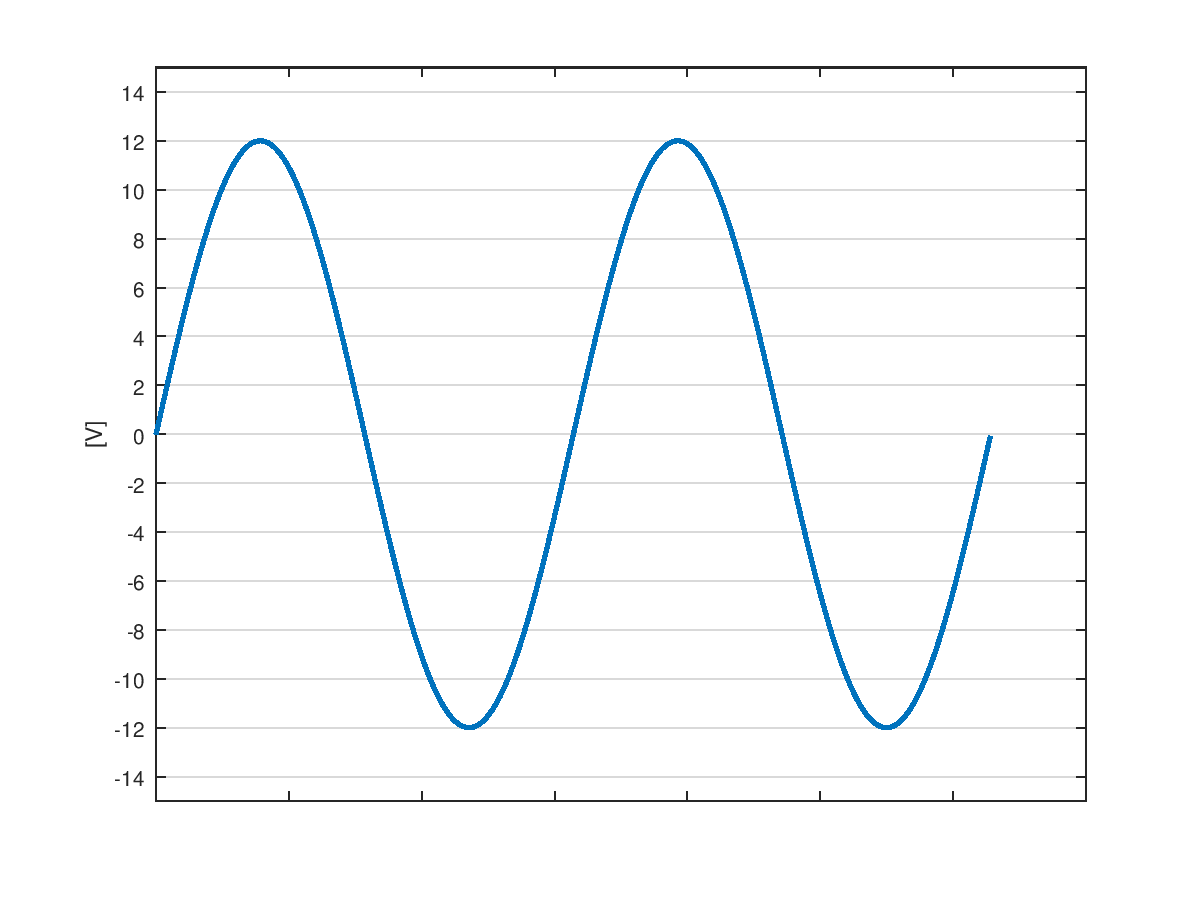
\includegraphics[width=.8\textwidth]{sinus.png}
    % x=[0:0.01:2*2*pi];plot(x,12*sin(x), "linewidth", 2);set(gca,'YTick',-14:2:14, "ygrid", "on", "xticklabel",[]); ylabel("[V]")
    

}{

    Pour $|V_{in}| \geq 8V$, nous serons dans la même situation que la question précédente : $D_1$ passante et $D_2$ en avalanche.
    Dans cette configuration, la somme des tensions aux bornes des diodes (et donc aux bornes de la charge) est $1.2 V + 6.8 V = 8 V$.
    On peut donc observer une saturation à cette tension, comme illustré dans le graphe suivant.

    \begin{center}
    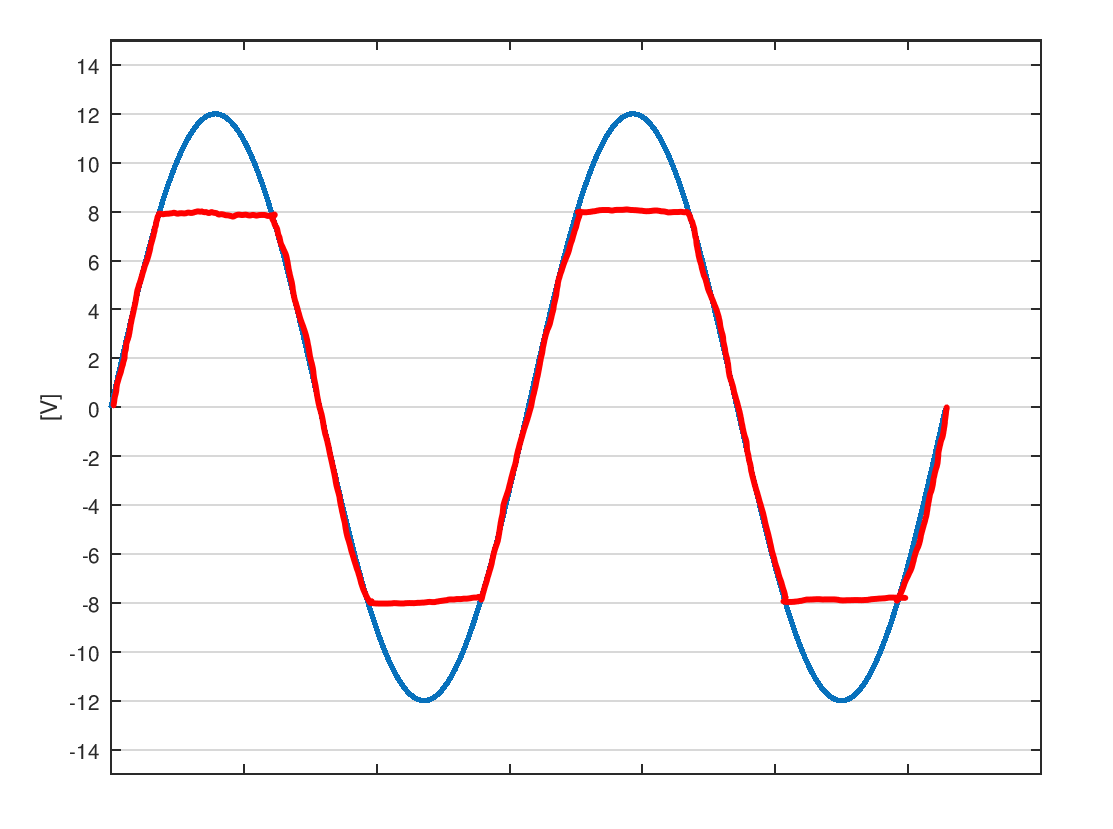
\includegraphics[width=.8\textwidth]{sinus_correction.png}
    \end{center}

    Attention, notez que la forme de $V_{out}$ (en rouge) devrait être légèrement atténuée.
    En effet, lorsque les diodes sont bloquantes ($|V_{in}| < 8 V$), $V_{out}$ est la tension d'un diviseur résistif formé de $R_1$ et $R_{ch}$ de rapport $\frac{9}{10}$.
}

\Question
{
    À quoi sert ce circuit ?
}{
    Ce circuit permet de limiter la tension de sortie et ainsi d'éviter que des piques de tension ne viennent endommager la charge.
    
    Ici la tension de sortie est limitée à $ \pm 8~V $.
}


\subsection*{Datasheet diode $ 1N4740A $}
\fbox{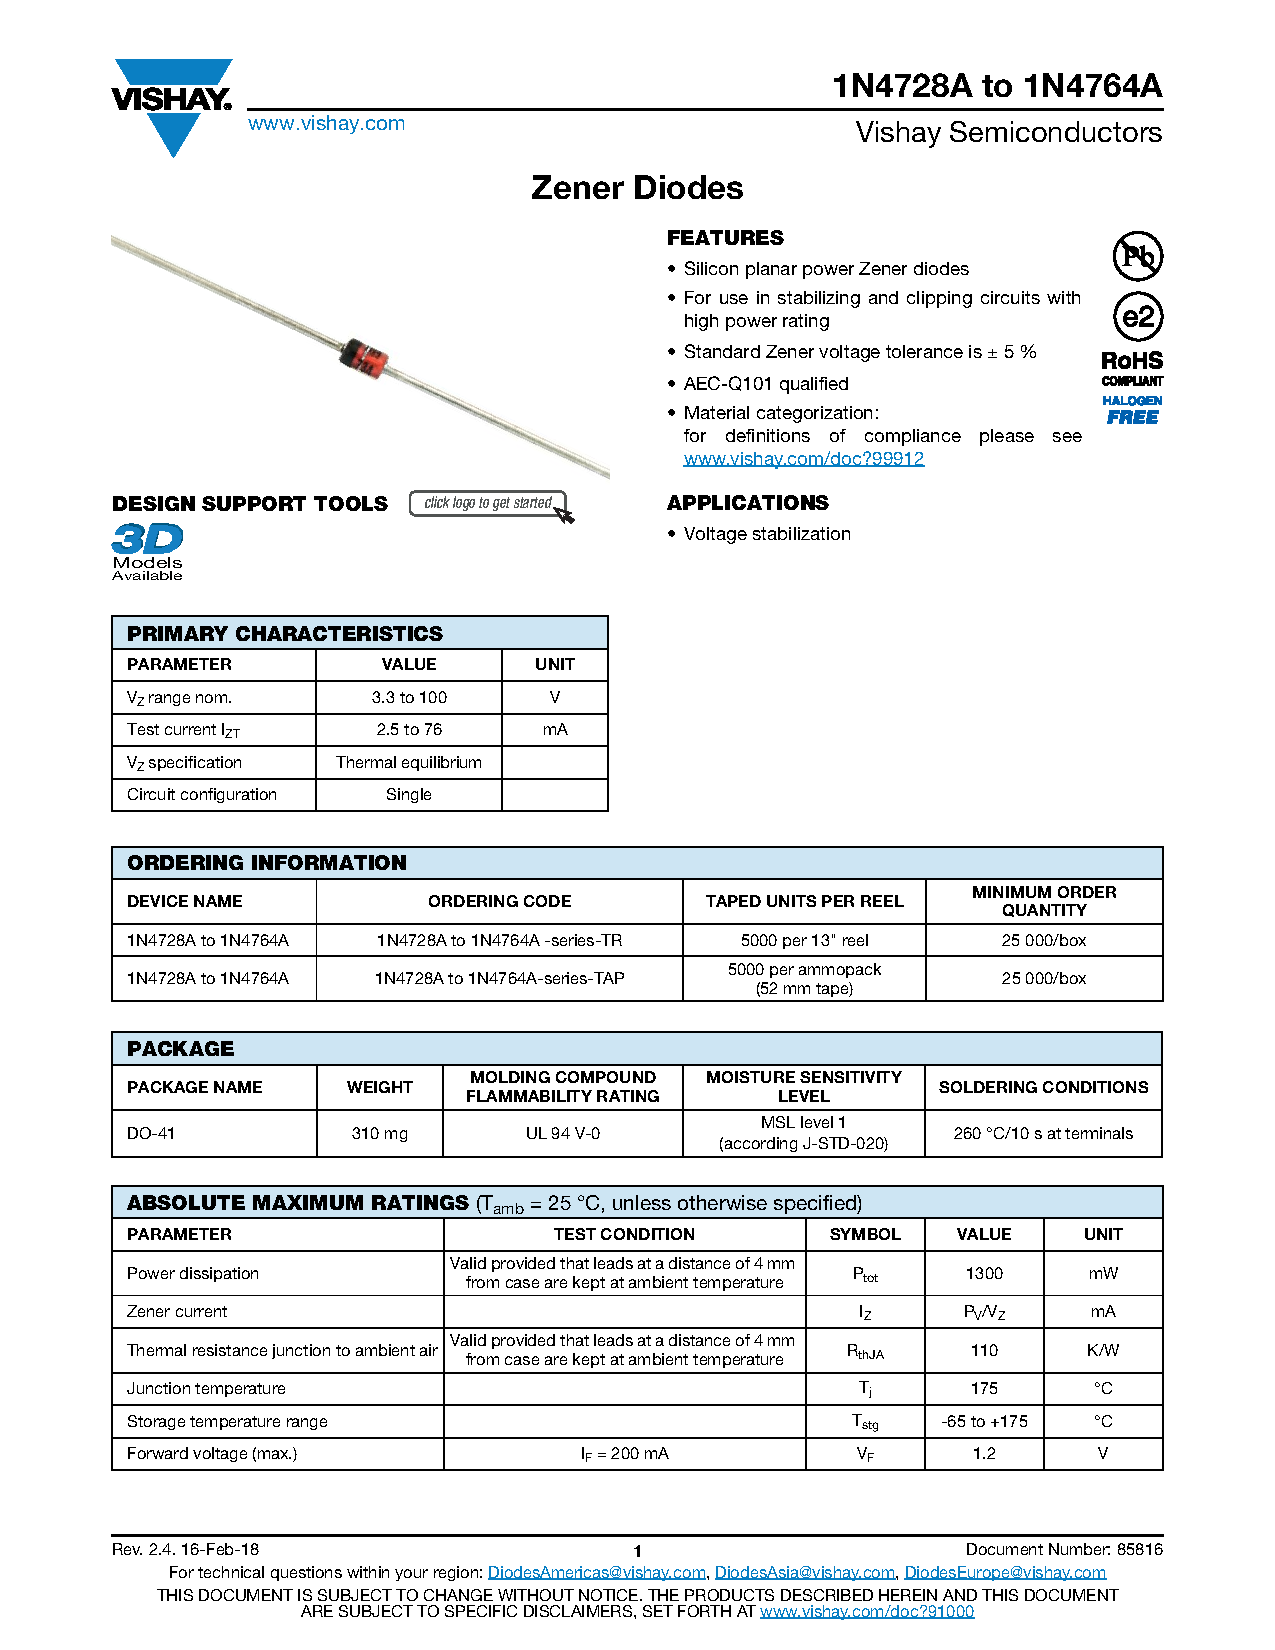
\includegraphics[page=1, width=\textwidth]{datasheet_diode.pdf}} \newpage
\fbox{\includegraphics[page=2, width=\textwidth]{datasheet_diode.pdf}}




\end{document}
